\section{ARIMA}

Time series forecasting is essential in many fields like finance, economics, climate science, and healthcare. One of the most widely used models for such forecasting is the ARIMA model, which stands for AutoRegressive Integrated Moving Average.

\subsection*{What is ARIMA?}

ARIMA combines three components:
\begin{itemize}
    \item \textbf{AR (AutoRegressive):} Uses past values to predict the current value.
    \item \textbf{I (Integrated):} Applies differencing to make the series stationary (removing trends).
    \item \textbf{MA (Moving Average):} Uses past forecast errors to predict current values.
\end{itemize}

The model is denoted as ARIMA(p, d, q):
\begin{itemize}
    \item \( p \): Number of autoregressive terms.
    \item \( d \): Number of times the data is differenced.
    \item \( q \): Number of lagged forecast errors.
\end{itemize}

\subsection*{Key R Libraries for ARIMA Modeling}

To apply ARIMA models in R, several useful packages are available that simplify the process of time series modeling and forecasting:
\begin{itemize}
    \item \textbf{stats} \\
    This is a base R package that provides the \texttt{arima()} function, which allows you to manually fit ARIMA models by specifying the values of \(p\), \(d\), and \(q\). It also includes the classic \texttt{ts()} function for creating time series objects.
    \begin{verbatim}
    fit <- arima(data, order = c(1,1,1))
    \end{verbatim}
    
    \item \textbf{forecast} \\
    Developed by Rob J Hyndman, this package provides the convenient \texttt{auto.arima()} function, which automatically selects the best ARIMA model based on AIC/BIC values. It also offers functions for forecasting, plotting, and evaluating models.
    \begin{verbatim}
    library(forecast)
    fit <- auto.arima(data)
    forecasted <- forecast(fit, h = 12)
    plot(forecasted)
    \end{verbatim}
    
    \item \textbf{tseries} \\
    This package supports time series analysis and includes the \texttt{adf.test()} for checking stationarity using the Augmented Dickey-Fuller test — a crucial step before fitting an ARIMA model.
    \begin{verbatim}
    library(tseries)
    adf.test(data)
    \end{verbatim}
    
    \item \textbf{ggplot2} \\
    While not specific to ARIMA, \texttt{ggplot2} is often used alongside these packages to create visually appealing time series plots and diagnostic graphs.
    \begin{verbatim}
    library(ggplot2)
    autoplot(forecasted)
    \end{verbatim}
\end{itemize}

These libraries together make it easy to preprocess, model, forecast, and visualize time series data in R using ARIMA.

\subsection*{ARIMA with R}

\textbf{Step 1: Data Aggregation}\\\\
We filtered the dataset for the district “Arghakhanchi,” extracted the year from the date, and computed the average temperature for each year.
\begin{verbatim}
temp_data <- climate_data %>% 
  filter(District == "Arghakhanchi") %>%
  mutate(Year = year(Date)) %>%  # Extract year from Date column
  group_by(Year) %>% 
  summarise(avg_temp = mean(Temp_2m, na.rm = TRUE)) %>%
  ungroup()
\end{verbatim}

Explanation of Parameters:
\begin{itemize}
    \item \texttt{Temp\_2m}: Daily temperature measured 2 meters above the ground.
    \item \texttt{na.rm = TRUE}: This argument removes any missing (NA) values during the computation of the mean, ensuring that incomplete data does not distort the result.
\end{itemize}

\textbf{Step 2: Time Series Conversion}\\\\ 
We converted the aggregated data into a time series object suitable for ARIMA modeling.
\begin{verbatim}
temp_ts <- ts(temp_data$avg_temp, 
start = min(temp_data$Year), frequency = 1) # Yearly data
\end{verbatim}

\textbf{Step 3: Fit ARIMA Model} \\ \\
We used the \texttt{auto.arima()} function, which automatically identifies the best ARIMA(p,d,q) model based on AICc (corrected Akaike Information Criterion).
\begin{verbatim}
model <- auto.arima(temp_ts)
summary(model)
\end{verbatim}

Explanation of Parameters:
\begin{itemize}
    \item \(p\): Autoregressive order — how many past values influence the present.
    \item \(d\): Differencing — how many times the data needs to be differenced to achieve stationarity.
    \item \(q\): Moving average order — how many past error terms influence the present.
\end{itemize}

\textbf{Step 4: Forecasting the Next 10 Years} \\ \\
We used the fitted model to forecast future average annual temperatures.
\begin{verbatim}
forecast_temp <- forecast(model, h = 10)
\end{verbatim}

Explanation of Parameters:
\begin{itemize}
    \item \(h = 10\): Forecast horizon — predicts for the next 10 time points (years).
\end{itemize}

\textbf{Step 5: Visualization of Forecast}\\ \\ 
We used \texttt{autoplot()} to visualize the forecast with confidence intervals.
\begin{verbatim}
autoplot(forecast_temp) + 
  ggtitle("10-Year Forecast of Average Annual Temperature\n(Arghakhanchi)") + 
  ylab("Average Temperature") + 
  xlab("Year")
\end{verbatim}

\begin{figure}[h]
\centering
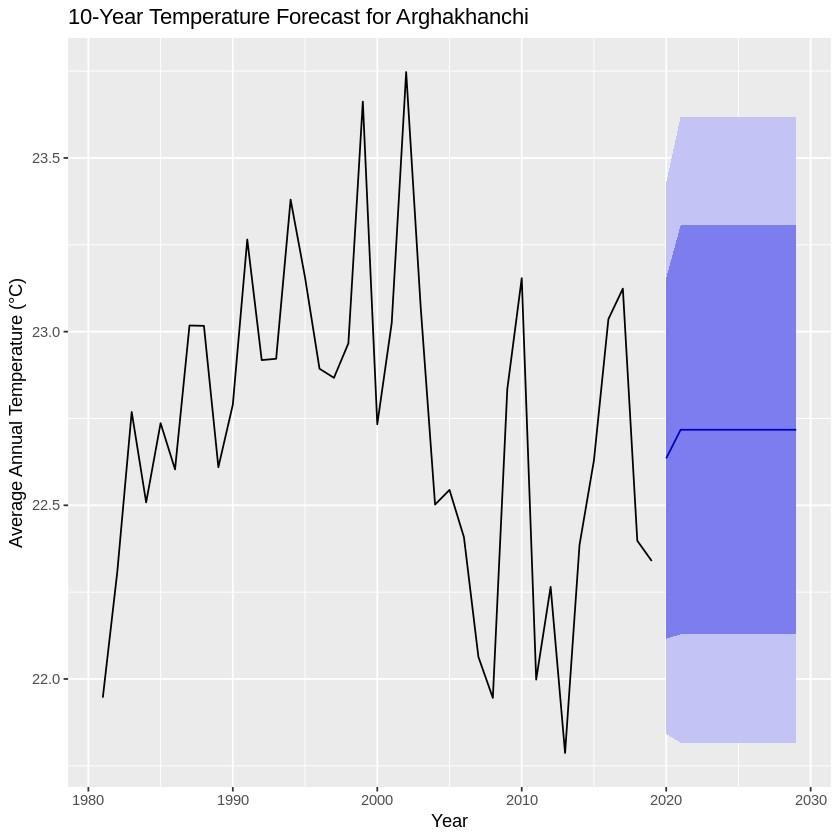
\includegraphics[width=0.5\textwidth]{figures/Arima.jpg}
\caption{10-Year Forecast of Average Annual Temperature in Arghakhanchi}
\end{figure}

\subsubsection*{Interpretation}
The shaded regions represent 80\% and 95\% confidence intervals. The solid line is the forecasted average temperature. The ARIMA model suggests expected trends based on past yearly averages and can guide climate planning or policy recommendations.
